%!TEX root = ../thesis.tex

\chapter{深对流对氮氧化物垂直分布的影响} \label{sec:effects_on_nox_profile}

由第\ref{chapter:PE}章分析可知,将卫星观测所得的NO$_2$柱浓度与闪电数据相结合,
可以得出LNO$_2$的柱浓度和产率,然而无法直接获得NO$_2$的垂直分布。
虽然飞机观测试验可以得到对流周围尤其是出流区的NO$_2$垂直分布\citep{Barth.2019},
但是无法获得对流云内的NO$_2$。
目前为止,有两种方法可获得对流云内的NO$_2$:1)山顶测量,2)NO$_2$探空。
其中山顶测量只能针对局地的NO$_2$浓度进行探测,无法获得区域的NO$_2$垂直分布\citep{Reiter.1970,Wang.2021a},
而NO$_2$探空目前仍处于发展阶段,且主要集中于边界层内\citep{Sluis.2010},尚未开展针对对流层上层的测试和观测试验。
因此本章将采用云切片的方法(\ref{sec:cloud-slicing}节),利用TROPOMI针对不同高度深厚对流云的观测,得到云间的NO$_2$平均浓度。

本章余下部分按照以下方式组织:
\ref{sec:model_settings_gmi}节介绍MERRA2-GMI模式使用的数据及方案;
\ref{sec:no2_vcd_cld}节分析TROPOMI测得的中低纬度云上NO$_2$柱浓度分布;
\ref{sec:no2_profile}节在\ref{sec:no2_vcd_cld}节的基础上,利用云切片方法计算1$^{\circ}$ $\times$ 1$^{\circ}$ 网格内不同高度的NO$_2$平均浓度,并与模拟的LNO$_2$排放廓线进行对比分析;
\ref{sec:lnox_affects_tropomi}节选取中国东南部的对流个例,利用WRF-Chem的高分辨率模拟探讨LNO$_2$对对流系统不同位置的TROPOMI NO$_2$柱浓度产品的影响,
最后是本章小结。



\section{模式设置} \label{sec:model_settings_gmi}

\ref{sec:no2_vcd_cld}节中MERRA2-GMI的模拟包括来自化石燃料、生物燃料、生物质燃烧和生物排放的NO、CO 和其他NMVOC。
除此之外,NO的排放还源自于闪电和土壤。
化石燃料和生物燃料的排放是取自测量大气成分和气候特大城市--放大环境(MACCity)清单\citep{Granier.2011},
利用十年大气化学和气候模式比较项目(ACCMIP)插值到每年的排放量并应用季节性比例因子\citep{Lamarque.2010}。
生物质燃烧排放来自全球火灾排放数据集(GFED)第4版\citep{Giglio.2013}。
生物来源使用自然界气体和气溶胶排放模型 [MEGAN,\citet{Guenther.1999}]
在线计算异戊二烯和其他生物化合物的排放量,并响应于MERRA2-GMI 气象场。
土壤的NO排放基于\citet{Yienger.1995},也响应于MERRA-2气象场。
闪电NO的排放使用 MERRA-2 中对流层中层的去趋势累积质量通量\citep{Allen.2010},
并受 OTD LIS闪电气候学的季节性约束\citep{Cecil.2014},
将全球平均比例因子应用于去趋势的累积质量通量,使得模拟每年的全球平均闪电 NO$_x$产量为 6.5 Tg N。
\ref{sec:lnox_affects_tropomi}节中的WRF-Chem模拟设置见\ref{sec:model_settings_china}节。

% \subsection{气象及化学设置}
% \subsection{闪电参数化}

% \section{模式评估}


\begin{figure}[H]
    \centering
    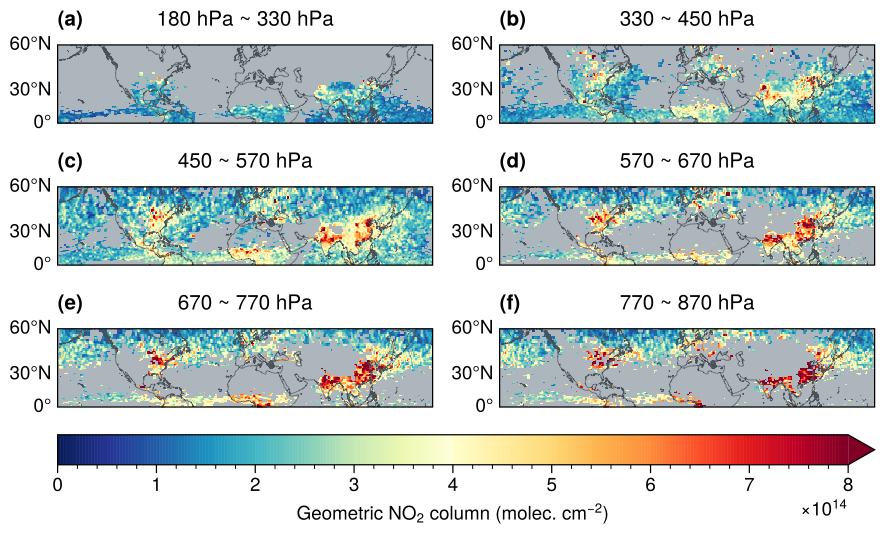
\includegraphics[width=0.9\textwidth]{./figures/no2geo_tropomi.png}
    \caption{
    2019年6--8月北半球中低纬度TROPOMI观测的云上NO$_2$柱浓度分布图:
    高云[(a)对流层顶 --330 hPa 和(b)330--450 hPa],
    中云 [(c)450--570 hPa 和(d)570--670 hPa],
    及低云 [(e) 670--770 hPa 和(f)770--870 hPa]。 \\
    Figure \ref{fig:no2geo_tropomi}. NO$_2$ above cloud at the middle-low latitudes for June--August in 2019:
    High clouds [(a) tropopause--330 hPa, (b) 330--450 hPa],
    middle clouds [(c) 450--570 hPa, (d) 570--670 hPa],
    and low clouds [(e) 670--770 hPa, (f) 770--870 hPa].
    }
    \label{fig:no2geo_tropomi}
\end{figure}

\section{结果与讨论}

\subsection{云上二氧化氮柱浓度的分布} \label{sec:no2_vcd_cld}

图\ref{fig:no2geo_tropomi}为TROPOMI观测的2019年中低纬度云上NO$_2$柱浓度分布图,
气压区间分别为对流层顶--330 hPa、330--450 hPa、
450--570 hPa、570--670 hPa、670--770 hPa和770--870 hPa。
其中对流层顶--330 hPa和330--450 hPa的云上NO$_2$高值区位于北美东北部、中国沿海地区、中国华北地区、墨西哥、
孟加拉国、尼泊尔、新德里、非洲中部和热带辐合带,
这些地区与图\ref{fig:no2_ltngcount}c中的闪电高值区相对应。
前人研究表明,中低纬LNO$_2$的峰值分布在100--500 hPa之间\citep{Pickering.1988,Ott.2010,Luo.2017},
故对流层顶--450 hPa的云上NO$_2$包含了LNO$_2$的贡献。
然而TROPOMI的晴空NO$_2$平均柱浓度产品显示这些地区属于NO$_2$高污染区(图\ref{fig:no2_ltngcount}b),
所以云压处于对流层上层的NO$_2$柱浓度也有来自深对流垂直输送的污染NO$_2$。
中云(450--670 hPa)的云上NO$_2$柱浓度有效数据更多,
其高值区包含了高云(对流层顶--450 hPa)的云上NO$_2$柱浓度高值区。
其中污染NO$_2$的贡献更为明显,与晴空NO$_2$平均柱浓度产品分布更为接近,
如中国东部、欧洲和北美东北部的工业源以及非洲中部的生物质燃烧。
污染物排放在低云(670--870 hPa)的云上NO$_2$柱浓度分布中最为明显,然而由于热带地区云顶较高,有效数据更少。


\begin{figure}[H]
    \centering
    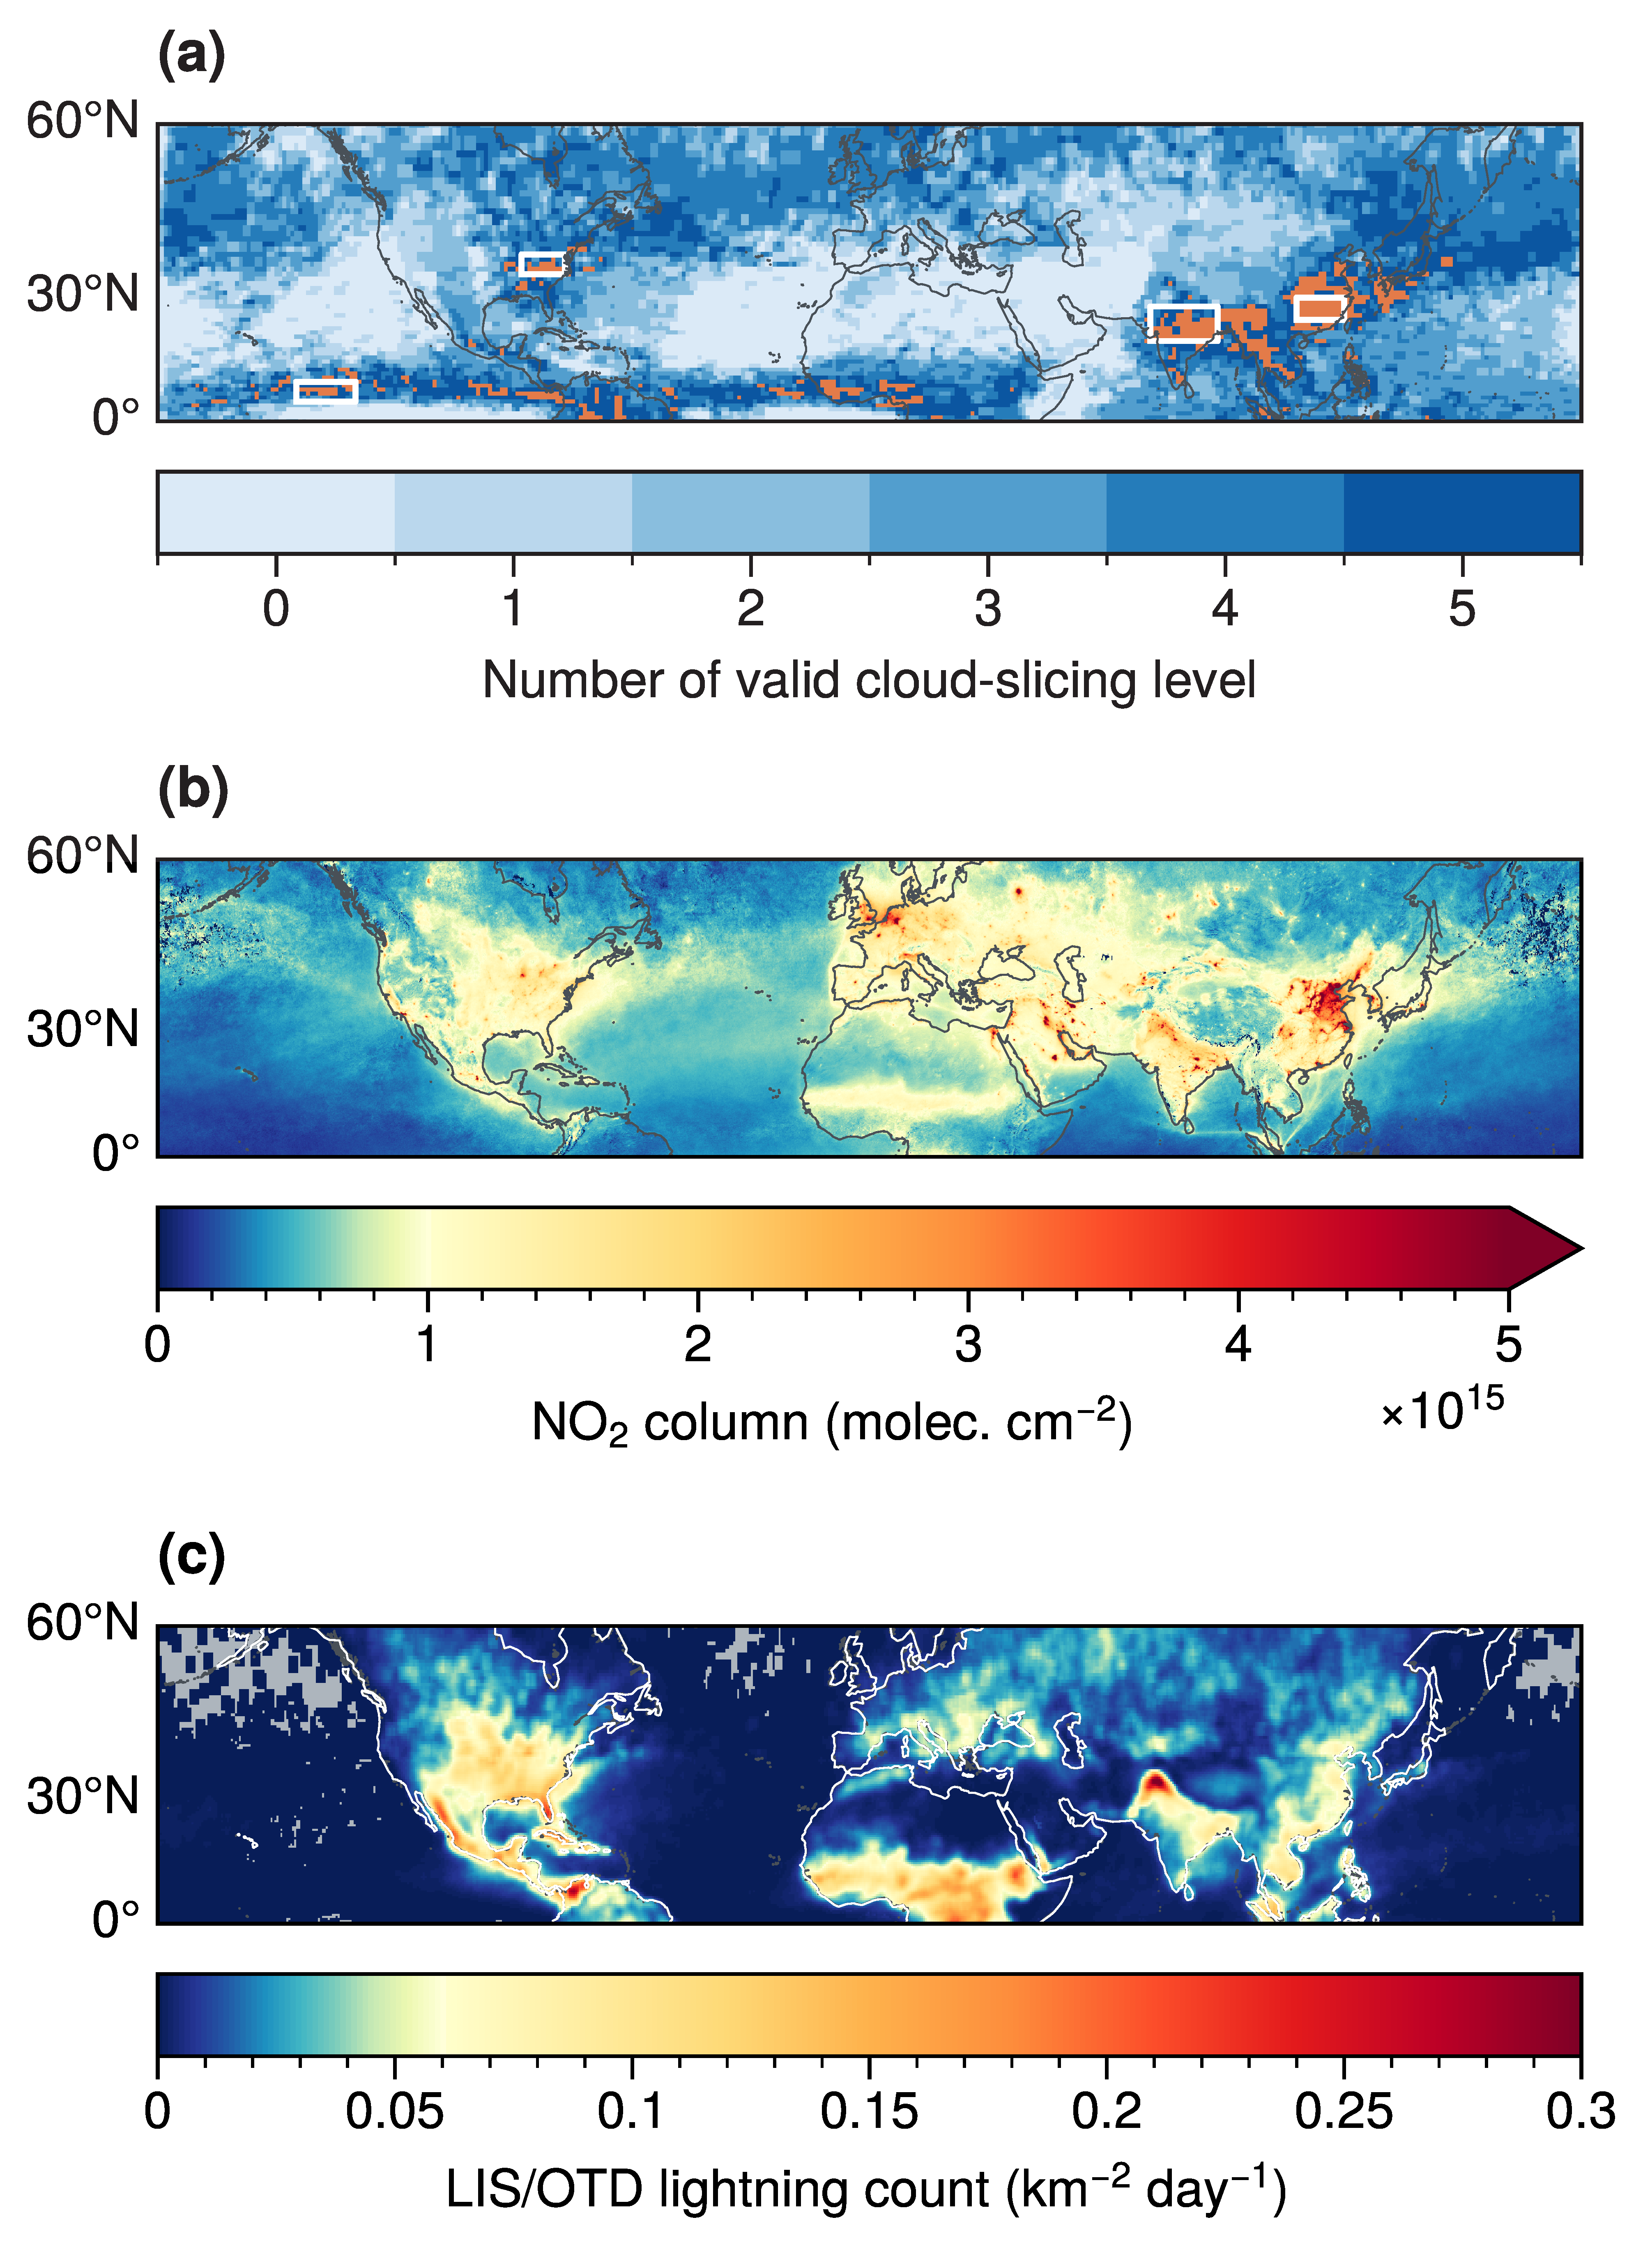
\includegraphics[width=0.7\textwidth]{./figures/no2_ltngcount.png}
    \caption{
    (a)云切片的总有效气压层数,层数$\leq$ 5为蓝色,= 6 为橙色,白色方框为NO$_2$廓线选区(图\ref{fig:utno2_profile});
    (b)2019--2021年中低纬度夏季(6--8月)TROPOMI测得的NO$_2$平均柱浓度;
    (c)1995--2014年中低纬度夏季(6--8月)LIS/OTD的闪电密度产品。 \\
    Figure \ref{fig:no2_ltngcount}. (a) Number of total valid cloud-slicing pressure levels.
    Grids with number of levels $\leq$ 5 and = 6 are filled in blue and orange, respectively.
    White rectangles are selections for NO$_2$ profiles (Fig. \ref{fig:utno2_profile}).
    (b) The average TROPOMI NO$_2$ column densities at the middle-low latitudes for June--August in 2019--2021.
    (c) The average LIS/OTD lightning flash rates at the middle-low latitudes for June--August in 1995--2014.
    }
    \label{fig:no2_ltngcount}
\end{figure}

\subsection{二氧化氮的垂直分布} \label{sec:no2_profile}


上节得到的云上NO$_2$为对流层NO$_2$柱浓度,柱底为云的中心气压,
通过\ref{sec:cloud-slicing}章的云切片算法可进一步得到每层的NO$_2$浓度,即NO$_2$廓线。
图\ref{fig:utno2_tropomi}为2019年6--8月不同高度的NO$_2$平均浓度。
与图\ref{fig:no2geo_tropomi}的云上NO$_2$柱浓度不同,
高云处的NO$_2$浓度(图\ref{fig:utno2_tropomi}a,b)高于中云(图\ref{fig:utno2_tropomi}c,d)。
其中陆地上对流层顶--330 hPa间的NO$_2$浓度为330--450 hPa间的$\sim$1.2倍,为450--570 hPa间的$\sim$2倍,
而570 hPa以下(图\ref{fig:utno2_tropomi}d--f)陆地上的NO$_2$浓度逐渐上升。
该现象与前人的模式模拟和飞机观测结果相符:LNO$_2$在对流层上层占主导,
而人为污染NO$_2$在对流层下层占主导\citep{Pickering.1996,Ott.2010,Laughner.2017}。


\begin{figure}[H]
    \centering
    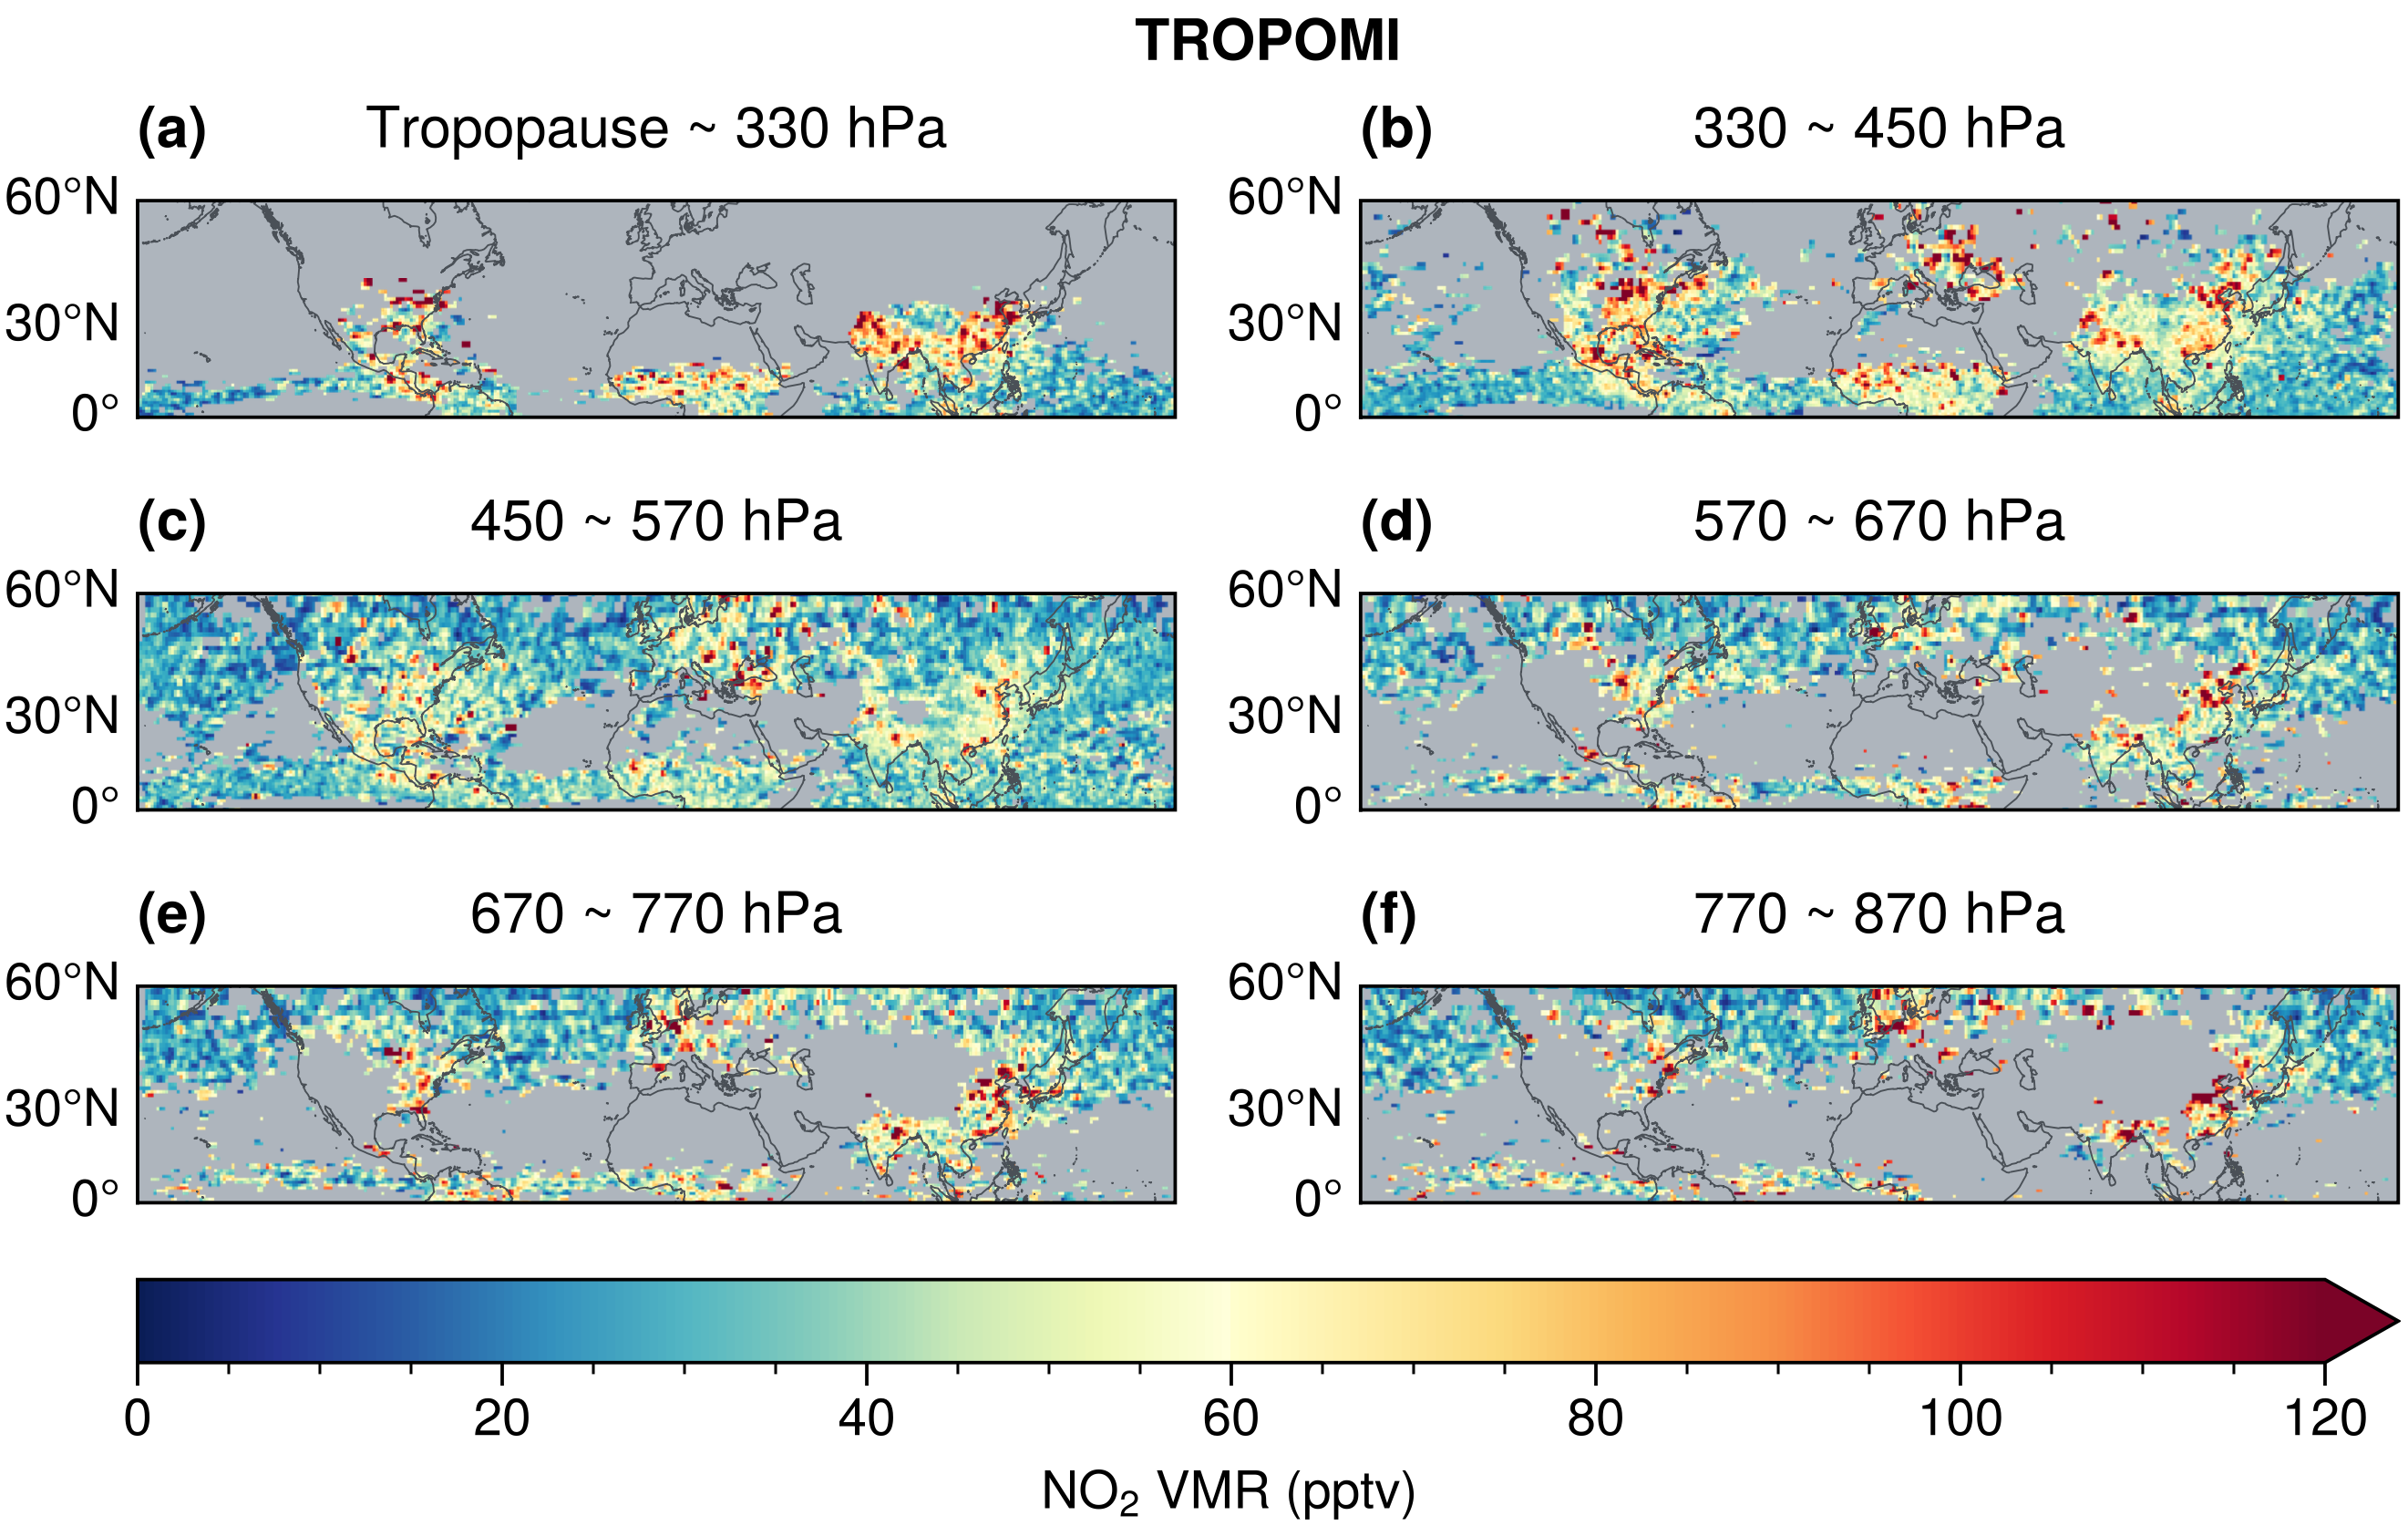
\includegraphics[width=0.9\textwidth]{./figures/utno2_tropomi.png}
    \caption{
    TROPOMI云切片算法所得的2019年6--8月北半球中低纬度NO$_2$浓度分布图。 \\
    Figure \ref{fig:utno2_tropomi}. The NO$_2$ vertical mixing ratios derived from the cloud-slicing results of TROPOMI NO$_2$ observations at the northern middle-low latitudes for June--August in 2019.
    }
    \label{fig:utno2_tropomi}
\end{figure}

为了进一步分析LNO$_2$在其中的作用,我们首先将各个高度层的TROPOMI观测结果与MERRA2-GMI的模式结果相比较,
接着选取TROPOMI云切片各层均有有效数据的区域,结合过境期间模拟的LNO$_2$排放速率垂直分布进行廓线分析。
图\ref{fig:utno2_merra2}为2019年6--8月与TROPOMI对应的MERRA2-GMI NO$_2$模拟结果,
% 由两者浓度之差(TROPOMI - MERRA2-GMI,图\ref{fig:utno2_delta})可知,无论位于陆地还是海洋,MERRA2-GMI较TROPOMI存在20--80 pptv的低估,
图\ref{fig:utno2_delta}为两者浓度之差(TROPOMI - MERRA2-GMI)的分布图。
其中海洋上的误差可能由TROPOMI NO$_2$反演过程中低估的平流层NO$_2$柱浓度或高估的辐射强度所导致\citep{VanGeffen.2020}。

具体而言,高云间的NO$_2$正误差为28 $\pm$ 19 pptv,
% 即高云间MERRA2-GMI模拟的NO$_2$比TROPOMI的观测值低25\%,
主要位于北美、东欧以及亚洲东部沿海(图\ref{fig:utno2_delta}a,b),
这意味着MERRA2-GMI全球模式中参数化对流垂直传输污染物的强度可能偏低。
而高云间的NO$_2$负误差(-12 $\pm$ 11 pptv)位于美国中部、非洲中部以及青藏高原西南部。
美国中部和非洲中部的误差是由于MERRA2-GMI中的闪电参数化(对流层上层的向上云质量通量)高估了该区域的闪电总量,从而导致NO$_2$浓度偏大\citep{Allen.2002,Allen.2010}。
由LIS/OTD闪电观测数据(图\ref{fig:no2_ltngcount}c)可知,
青藏高原西南部闪电强度较弱,故模式的高估主要应来自于亚洲夏季风的污染物输送。

中云的云切片结果有效范围最广,总体上来看TROPOMI和MERRA2-GMI之间误差较低(18 $\pm$ 17 pptv),
且两者具有相似的高值区分布:北美、东欧、印度以及中国华北地区,这些地区与污染NO$_2$柱浓度高值区对应。
中云高度的NO$_2$可能来源有对流输送的地表污染和污染的出流区,如中国华北地区的NO$_2$高值传输至东部的黄海(其中一部分也来自于船舶排放)。
其中$>$ 40 pptv的正误差集中于南美洲北部、缅甸和泰国北部,由于这些地区地基NO$_2$观测资料稀缺,
所以该误差应归因于卫星反演误差还是模式NO$_x$排放源的不确定性,还有待进一步研究。
此外,中云的负误差结果在570--670 hPa更为明显(-10 $\pm$ 15 pptv),尤其是中国的华北地区,
考虑到MERRA2-GMI对流垂直输送强度较低,故使用的排放清单中NO$_x$排放量可能过高\citep{Ziemke.2019}。

\begin{figure}[H]
    \centering
    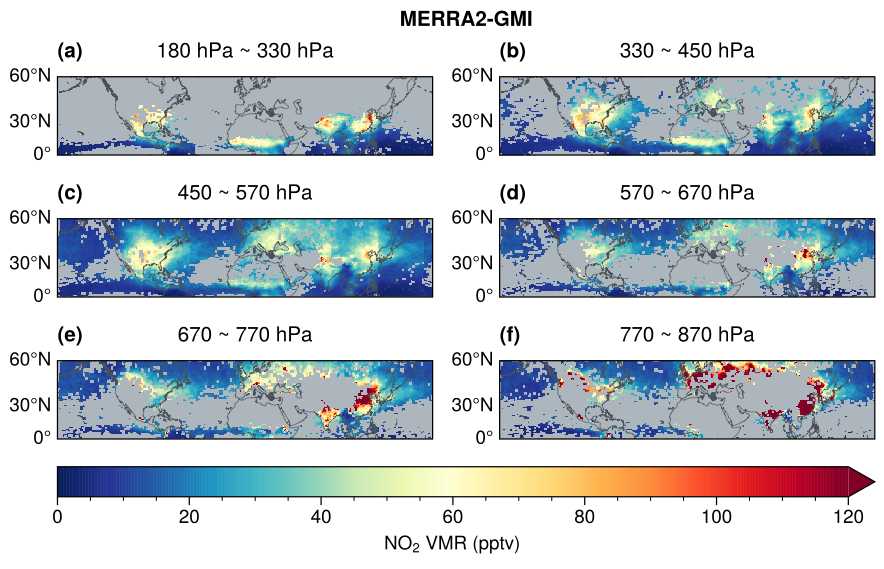
\includegraphics[width=0.9\textwidth]{./figures/utno2_merra2-gmi.png}
    \caption{
    同图\ref{fig:utno2_tropomi}但数据为MERRA2-GMI。 \\
    Figure \ref{fig:utno2_merra2}. Same as Fig. \ref{fig:utno2_tropomi} but for MERRA2-GMI.
    }
    \label{fig:utno2_merra2}
\end{figure}

低云的云切片NO$_2$高值区与中云结果类似,
总体上来看TROPOMI和MERRA2-GMI之间误差较大(15 $\pm$ 50 pptv),
在中国东部和印度北部的负误差最为明显($<$-100 pptv)。
前人研究表明,本研究中所用的几何AMF(AMF$_{geo}$,式\ref{eq:AMF_geo})在低云和污染条件下可达可见AMF(AMF$_{Vis}$,式\ref{eq:AMF_NO2Vis})的两倍\citep{BelmonteRivas.2015},然而这不足以解释中国东部地区的模拟值为观测值的3--5倍。
因此,该差异反映了MERRA2-GMI使用的MACCity排放清单在中国东部未能及时更新。


\begin{figure}[H]
    \centering
    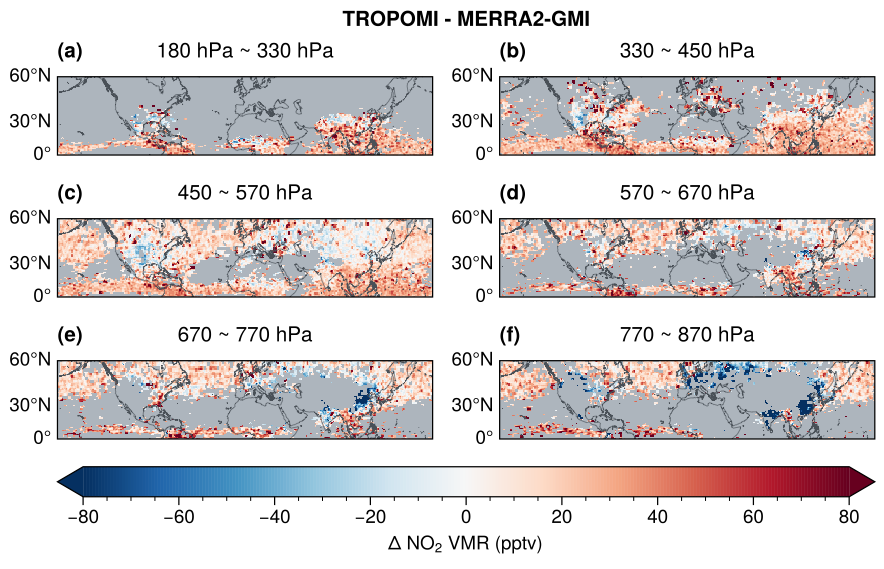
\includegraphics[width=0.9\textwidth]{./figures/utno2_delta.png}
    \caption{
    图\ref{fig:utno2_tropomi}与图\ref{fig:utno2_merra2}之差。 \\
    Figure \ref{fig:utno2_delta}. Differences between Fig. \ref{fig:utno2_tropomi} and Fig. \ref{fig:utno2_merra2}.
    }
    \label{fig:utno2_delta}
\end{figure}



除了各层NO$_2$浓度的地理分布之外,我们选取了区域内云切片有效层数为6层的格点
(分别位于中国南部、印度中部、美国东南部以及太平洋,图\ref{fig:no2_ltngcount}a),
进行TM5、MERRA2-GMI和TROPOMI的廓线对比分析,
其中TM5的NO$_2$廓线为TROPOMI官方产品使用的TM5全球模式先验廓线(包含TROPOMI同化)。
由于TROPOMI在太平洋清洁地区的高估,我们将云切片结果进行校正,即除以其与MERRA2-GMI和TROPOMI比例的平均值。
如图\ref{fig:utno2_profile}所示,太平洋清洁地区NO$_2$在对流层各层浓度分布均一(2.5--12.5 pptv),
中国南部和印度中部低层NO$_2$污染浓度高(200--300 pptv),而美国东南部低层NO$_2$浓度为50--100 pptv。
由于污染地区对流层低层TROPOMI NO$_2$浓度存在与图\ref{fig:utno2_delta}中类似的低估,故只比较三者在对流层中上层的NO$_2$浓度大小。


\begin{figure}[H]
    \centering
    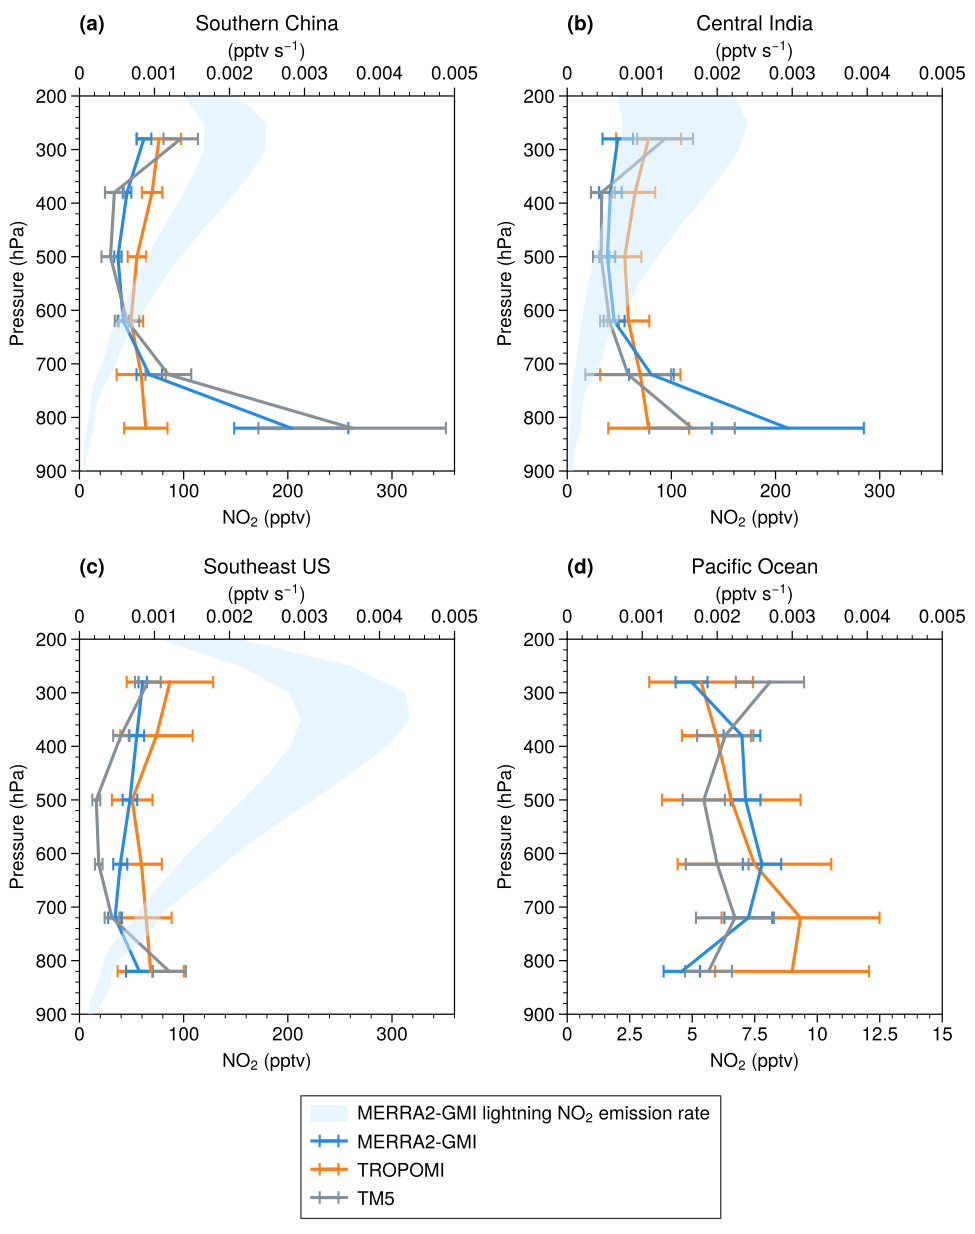
\includegraphics[width=0.9\textwidth]{./figures/utno2_profile.png}
    \caption{
    TM5(灰色)、MERRA2-GMI(蓝色)以及TROPOMI云切片算法(橙色)所得到的区域平均NO$_2$廓线:
    (a)中国南部、(b)印度中部、(c)美国东南部、(d)太平洋(区域示意图见图\ref{fig:no2_ltngcount}a)。
    浅蓝色填充部分为下午地方时2点的MERRA2-GMI闪电NO$_2$排放速率,
    其中廓线的误差棒和填充范围为平均值$\pm$标准差。\\
    Figure \ref{fig:utno2_profile}. Regional average NO$_2$ profiles obtained by TM5 (gray), MERRA2-GMI (blue), and TROPOMI cloud slice algorithm (orange).
    (a) southern China, (b) central India, (c) southeastern United States, and (d) Pacific Ocean
    (Definitions of region are shown in Fig. \ref{fig:no2_ltngcount}a).
    The light blue filled part is the MERRA2-GMI lightning NO$_2$ emission rate at local 2 p.m.,
    where the error bars and filled ranges of the profiles are the mean values $\pm$ standard deviations.
    }
    \label{fig:utno2_profile}
\end{figure}


对于中国南部、印度中部和美国东南部,NO$_2$廓线呈“C”形:NO$_2$首先随高度而下降,
在500--600 hPa存在转折点,进而浓度上升,在对流层顶--300 hPa达到峰值($\sim$80 pptv)。
总体来看,对流层中上层MERRA2-GMI和TM5的NO$_2$浓度相近,但均比TROPOMI的结果低,
表明模式中LNO$_2$或对流输送的污染NO$_2$存在低估,与前人的飞机探测和模式结果相符\citep{Laughner.2019a}。
具体而言,由于TM5的同化仅包含云上的信息,TM5的中上层拐点梯度更大,
其在对流层顶--330 hPa和330--450 hPa区间的NO$_2$浓度比TROPOMI的观测结果分别低10\%和50\%,
而MERRA2-GMI结果较TROPMI的结果低30\%。
此外,MERRA2-GMI在美国东南部的LNO$_2$排放速率为中国南部或印度中部的两倍,最上层的峰值浓度与TM5一致,
不同之处是浓度拐点降为700 hPa,该高度低于TM5和TROPOMI的500 hPa,
可能原因是MERRA2-GMI的美国东南部LNO$_2$排放廓线在对流层中低层权重过高。
总之,TROPOMI的观测结果和MERRA2-GMI/TM5的模拟结果在对流层中上层存在显著的一致性,
局部的差异表明云切片方法可以用来检验模式的对流垂直输送和水平输送能力、使用的排放源清单以及LNO$_x$的产量和分布。


\subsection{闪电氮氧化物对TROPOMI产品的影响}  \label{sec:lnox_affects_tropomi}

鉴于LNO$_2$在对流层中上层的主导地位和更长寿命,TROPOMI的NO$_2$产品可以用来研究不同区域LNO$_2$的分布。
然而官方的TROPOMI NO$_2$柱浓度产品所依赖的NO$_2$先验廓线并未详细考虑LNO$_2$的垂直分布,
所以我们接着针对中国东南部地区的对流系统(图\ref{fig:china_flash_scd}),
利用WRF-Chem的敏感性试验结果而非MERRA2-GMI资料,详细研究了LNO$_x$对官方NO$_2$柱浓度产品的影响。

为了探讨LNO$_x$对AMF$_{\ch{trop}}$和AMF$_{\ch{LNO_x}}$计算的重要性,
我们将LNO产率的上限700 mol NO 每闪电\citep{Ott.2010}应用于WRF-Chem ,并与500 mol NO 每闪电的结果进行对比。
接着我们通过独立替换对流层内三个不同高度区间的NO$_2$廓线:
对流层中层(MT,800--400 hPa)、
对流层上层(UT,400--150 hPa)和整个对流层(地表到对流层顶),
进行TROPOMI AMF的敏感性试验。
除非另有说明,否则后文AMF的变化是通过增加LNO$_x$获得。

如图\ref{fig:china_s5p_amf_diff}所示,
AMF变化主要由TROPOMI探测灵敏度高的对流层上层LNO$_x$所控制\citep{Beirle.2009,Laughner.2017},
且LNO$_x$产量在该高度达到峰值(图\ref{fig:china_nox_profile})。
虽然在三种廓线替换条件下AMF$_{\ch{LNO_x}}$均降低了5--40\%,
但AMF$_{\ch{trop}}$的变化($\Delta$AMF$_{\ch{trop}}$)具有区域特异性,
可根据闪电活动(图\ref{fig:china_flash_scd})对其进行分类:新生闪电区(MT $\Delta$AMF $<$ -20\%)、闪电下风向(MT $\Delta$AMF$_{\ch{trop}}$ $>$ 20\%)和闪电老化区(UT $\Delta$AMF$_{\ch{trop}}$ $>$ 20\%)。
结果表明,先验廓线中若考虑LNO$_2$,可导致新生闪电区的AMF$_{\ch{trop}}$降低23\%,而闪电下风向和闪电老化区的AMF$_{\ch{trop}}$增大60\%。

接着利用云高和敏感性试验结果,我们进一步分析了AMF$_{\ch{trop}}$在不同区域呈现不同变化的原因。
如图\ref{fig:china_amf_contribution}a所示,云层高于400 hPa时(云压 $<$ 400 hPa),
新生闪电区的像素上云辐射分数(f$_{\ch{effNO2}}$) $>$ 0.6,但闪电下风向和老化区均有低于400 hPa且f$_{\ch{effNO2}}$ $<$ 0.6的云层。
这与图\ref{fig:china_nox_profile}中的平均云压一致,并解释了为何UT $\Delta$AMF$_{\ch{trop}}$ > 20\% 在图\ref{fig:china_s5p_amf_diff}b$_i$和b$_{iii}$ 中存在,这也正表明了在闪电老化区估算LNO$_x$的可能性。
具体而言,LNO$_x$对$\Delta$AMF$_{\ch{trop}}$的贡献分为两部分:S$^{\ch{LNO_x}}_{\ch{tropNO2}}$/S$^{\ch{noLNO_x}}_{\ch{tropNO2}}$ 和 V$^{\ch{LNO_x}}_{\ch{tropNO2}}$/V$^{\ch{noLNO_x}}_{\ch{tropNO2}}$,
其中 LNO$_x$ 上标表示先验变量是开启 LNO$_x$排放(500 mol NO每闪电),而 noLNO$_x$ 代表关闭LNO$_x$排放。
这两个贡献是通过对式(\ref{eq:AMF1})和式(\ref{eq:AMF0})取对数,然后相减得到式(\ref{eq:delta_AMF}),其中下标$1$是开启LNO$_x$排放,下标$0$是关闭LNO$_x$排放。
这两部分可用于确定哪个参数控制$\Delta$AMF$_{\ch{trop}}$:增大的先验S$_{\ch{tropNO2}}$ 或先验 V$_{\ch{tropNO2}}$(图\ref{fig:china_amf_contribution}b--d)。
简而言之,图\ref{fig:china_amf_contribution}b--d中哪个比例的数值大,哪个占主导地位。
{
\abovedisplayskip=5pt%
\belowdisplayskip=5pt%
\begin{equation} \label{eq:AMF1}
\textrm{AMF}_1 = \frac{S_1}{V_1}
\end{equation}
\begin{equation} \label{eq:AMF0}
\textrm{AMF}_0 = \frac{S_0}{V_0}
\end{equation}
\begin{equation} \label{eq:delta_AMF}
\begin{split}
\textrm{log(AMF$_1$)} - \textrm{log(AMF$_0$)} & = \textrm{log}(\frac{S_1}{V_1}) - \textrm{log}(\frac{S_0}{V_0}) \\
                                              & = \textrm{log}(\frac{S_1}{S_0}) - \textrm{log}(\frac{V_1}{V_0})
\end{split}
\end{equation}
}

首先,如果将LNO$_2$包含在先验NO$_2$廓线中(图\ref{fig:china_s5p_amf_diff}c$_i$),
新生闪电区由于增大的先验V$_{\ch{NO2}}$(图 \ref{fig:china_amf_contribution}b),AMF$_{\ch{trop}}$将减小。
而新生闪电的下风向区域情况相反,无论选择哪一层替换NO$_2$廓线,
AMF$_{\ch{trop}}$均增大(图\ref{fig:china_s5p_amf_diff}a$_{i}$--c$_{i}$),
这是由于对流将LNO $_2$输送至云顶上方,并导致更大的先验 S$_{\ch{NO2}}$(图 \ref{fig:china_amf_contribution}c)。
对于2020年个例的老化闪电像素处,针对对流层上层的AMF$_{\ch{trop}}$结果增加$>$50 \%(图\ref{fig:china_s5p_amf_diff}b$_{iii}$)。
该现象证明了平流输送的对流层上层LNO$_2$和云作为屏障的重要作用,即导致先验S$_{\ch{NO$_2$}}$和先验V$_{\ch{NO2}}$之间的差异(图 \ref{fig:china_amf_contribution}d)。
尽管由于对流附近LNO$_2$的寿命较短,该差异小于其他两个区域,但它对于计算LNO$_x$ 仍然有用。
此外,考虑到LNO$_x$对AMF影响的区域性,我们需要在 TROPOMI NO$_2$ 的产品中更为详细地考虑LNO$_2$,尤其是在出流区域。
而TM5-MP 和 WRF-Chem NO$_2$ 廓线之间的比较(图 \ref{fig:china_nox_profile})也说明了可分辨的对流输送和LNO$_x$的重要性。



\begin{figure}[H]
    \centering
    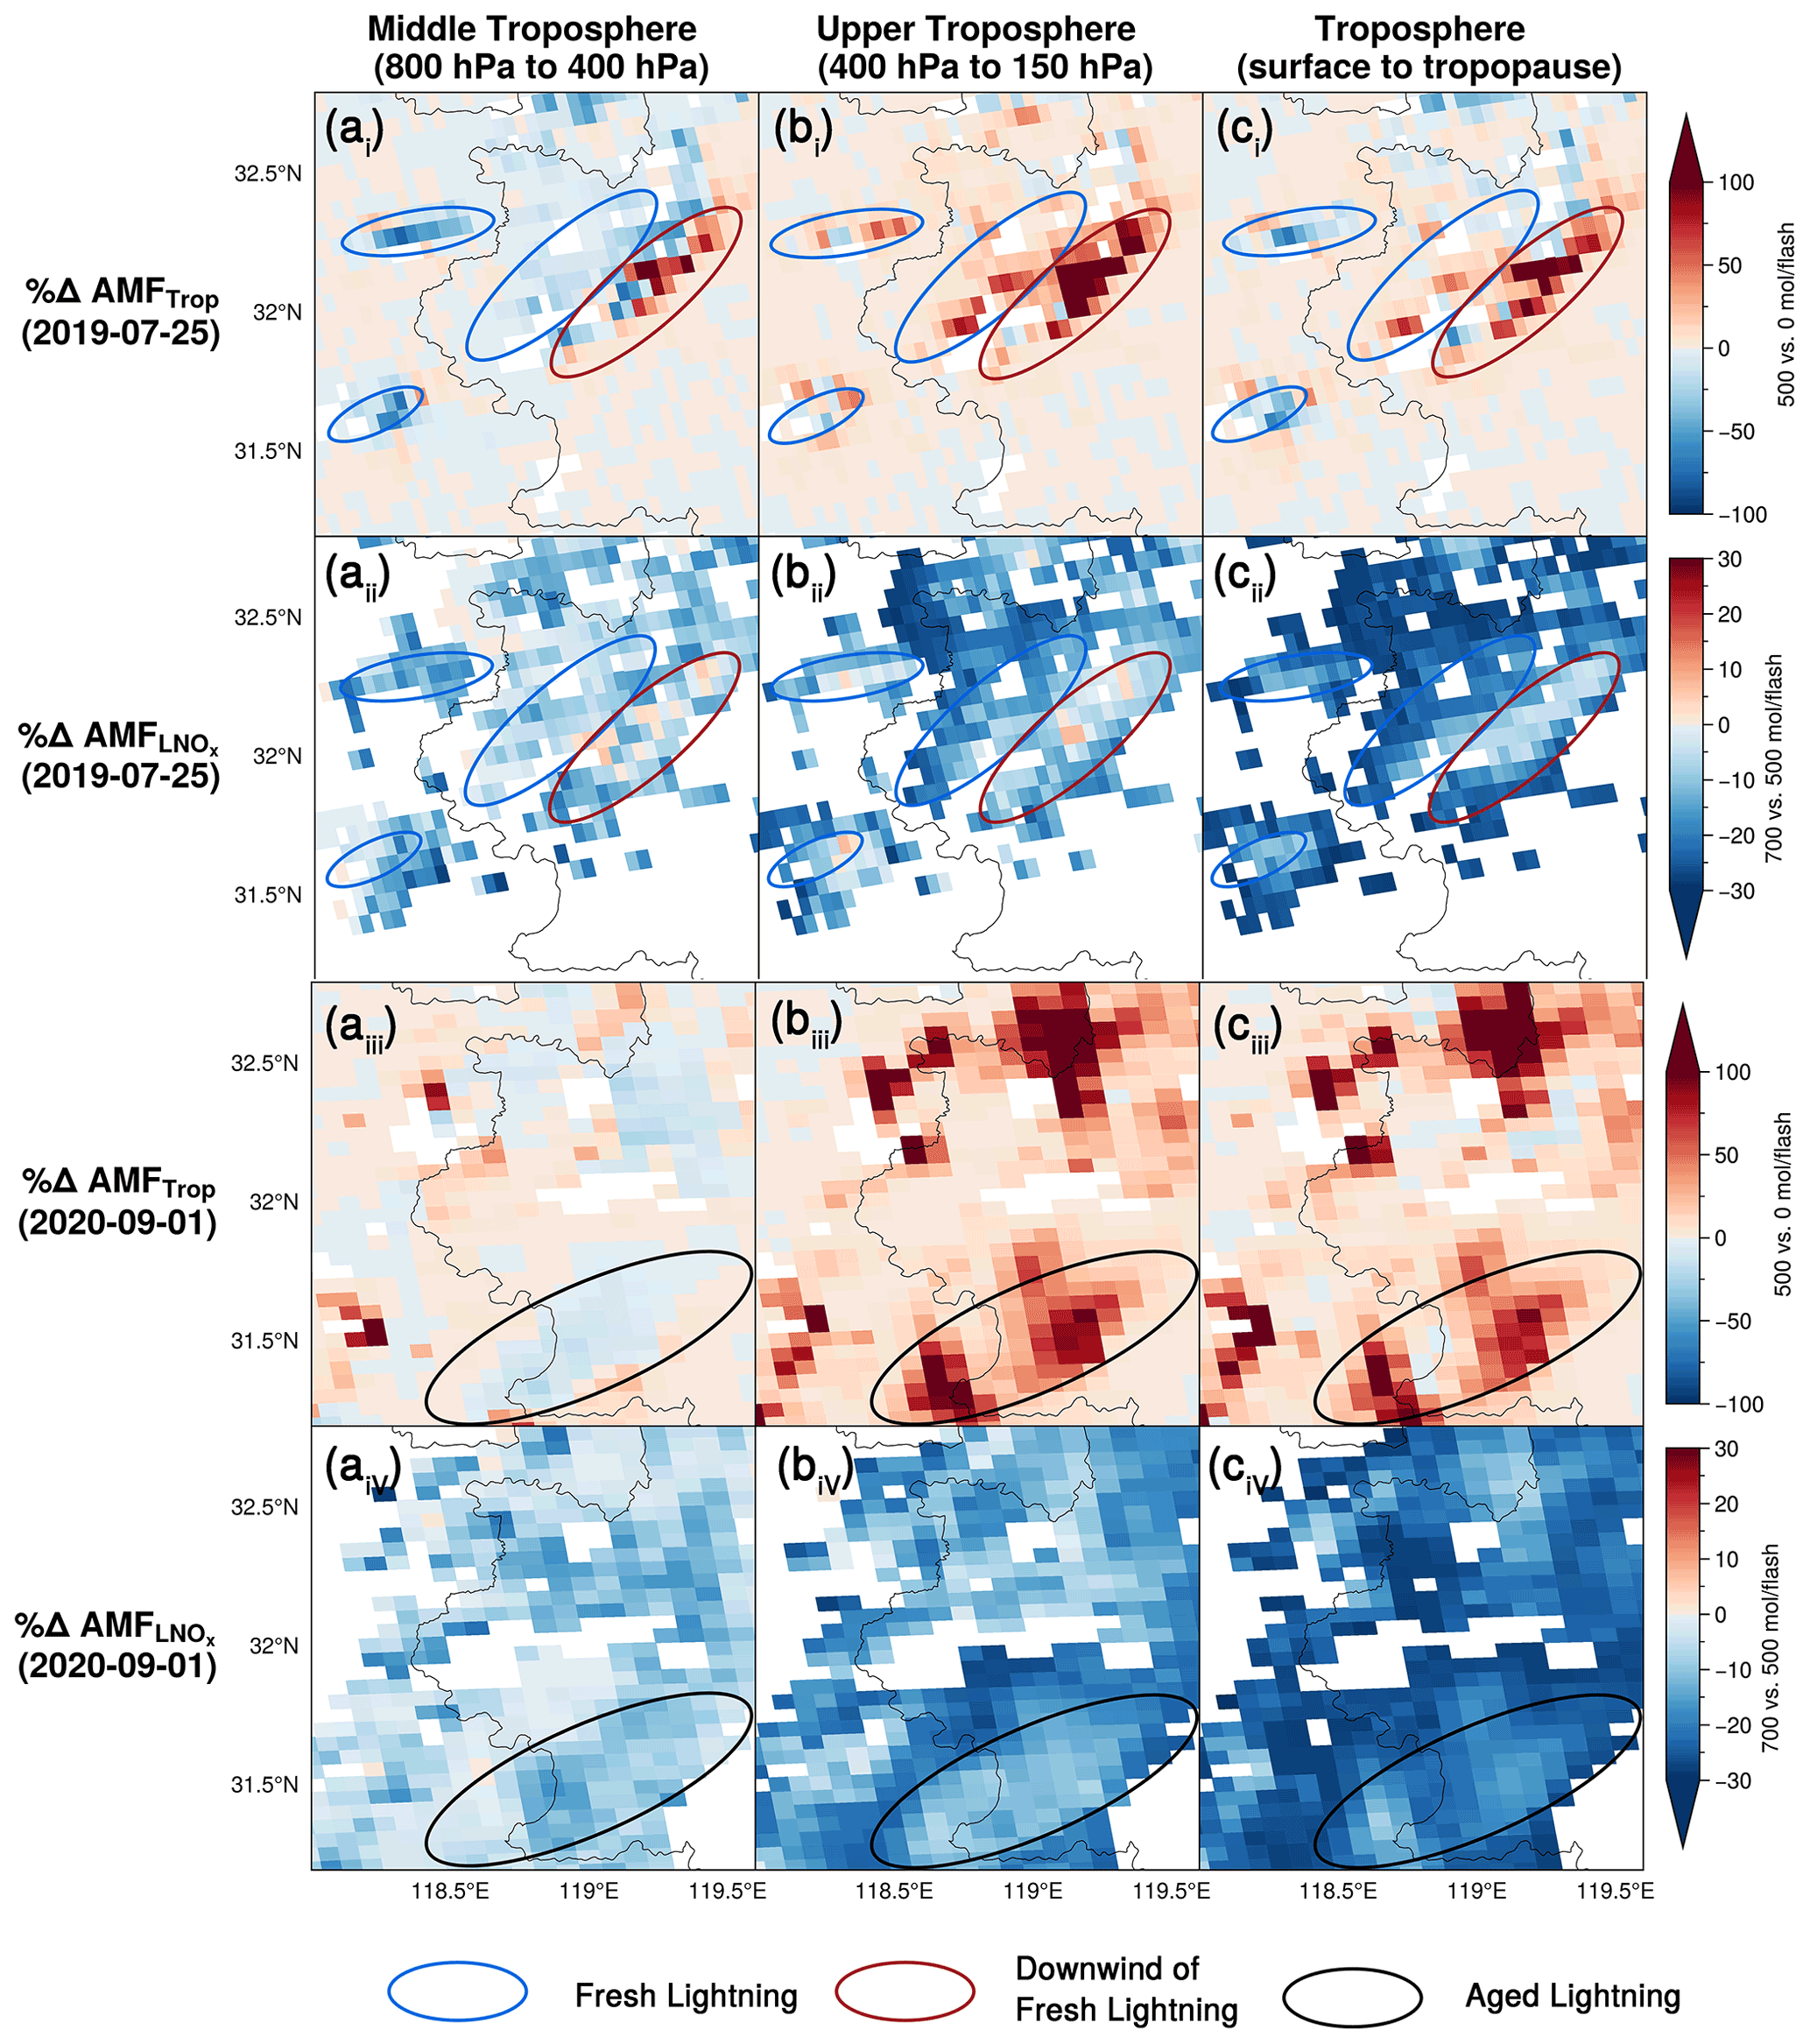
\includegraphics[width=0.9\textwidth]{./figures/china_s5p_amf_diff.png}
    \caption{
    通过替换三层的NO$_2$先验廓线,得到的大气质量因子(AMF)百分比差异。
    三层具体为:对流层中层(左)、对流层上层(中)和整个对流层(右)。
     $\Delta$AMF$_\textrm{trop}$ 是 500 mol NO/闪电得到的AMF$_\textrm{trop}$ 与 0 mol NO/闪电得到的AMF$_\textrm{trop}$之差。
     $\Delta$AMF$_\textrm{LNO$_x$}$ 是 700 mol NO/闪电得到的AMF$_\textrm{LNO$_x$}$ 与 500 mol NO/闪电得到的AMF$_\textrm{LNO$_x$}$之差。
     图中标注的三个椭圆区域为:新生闪电区(蓝色),闪电下风向(红色),和闪电老化区(黑色)。\\
    Figure \ref{fig:china_s5p_amf_diff}. The percent differences of AMFs by replacing the a priori NO$_2$ profiles at three layers:
    middle troposphere (left), upper troposphere (middle), and troposphere (right).
    $\Delta$AMF$_\textrm{trop}$ is the comparison of the AMF$_\textrm{trop}$ with 500 mol NO per flash relative to 0 mol NO per flash.
    $\Delta$AMF$_\textrm{LNO$_x$}$ is the comparison of the AMF$_\textrm{LNO$_x$}$ with 700 mol NO per flash relative to 500 mol NO per flash.
    Three regions are annotated: fresh lightning (blue),
    downwind of fresh lightning (red),
    and aged lightning (black).
    }
    \label{fig:china_s5p_amf_diff}
\end{figure}


\begin{sidewaysfigure}[!htbp]
    \centering
    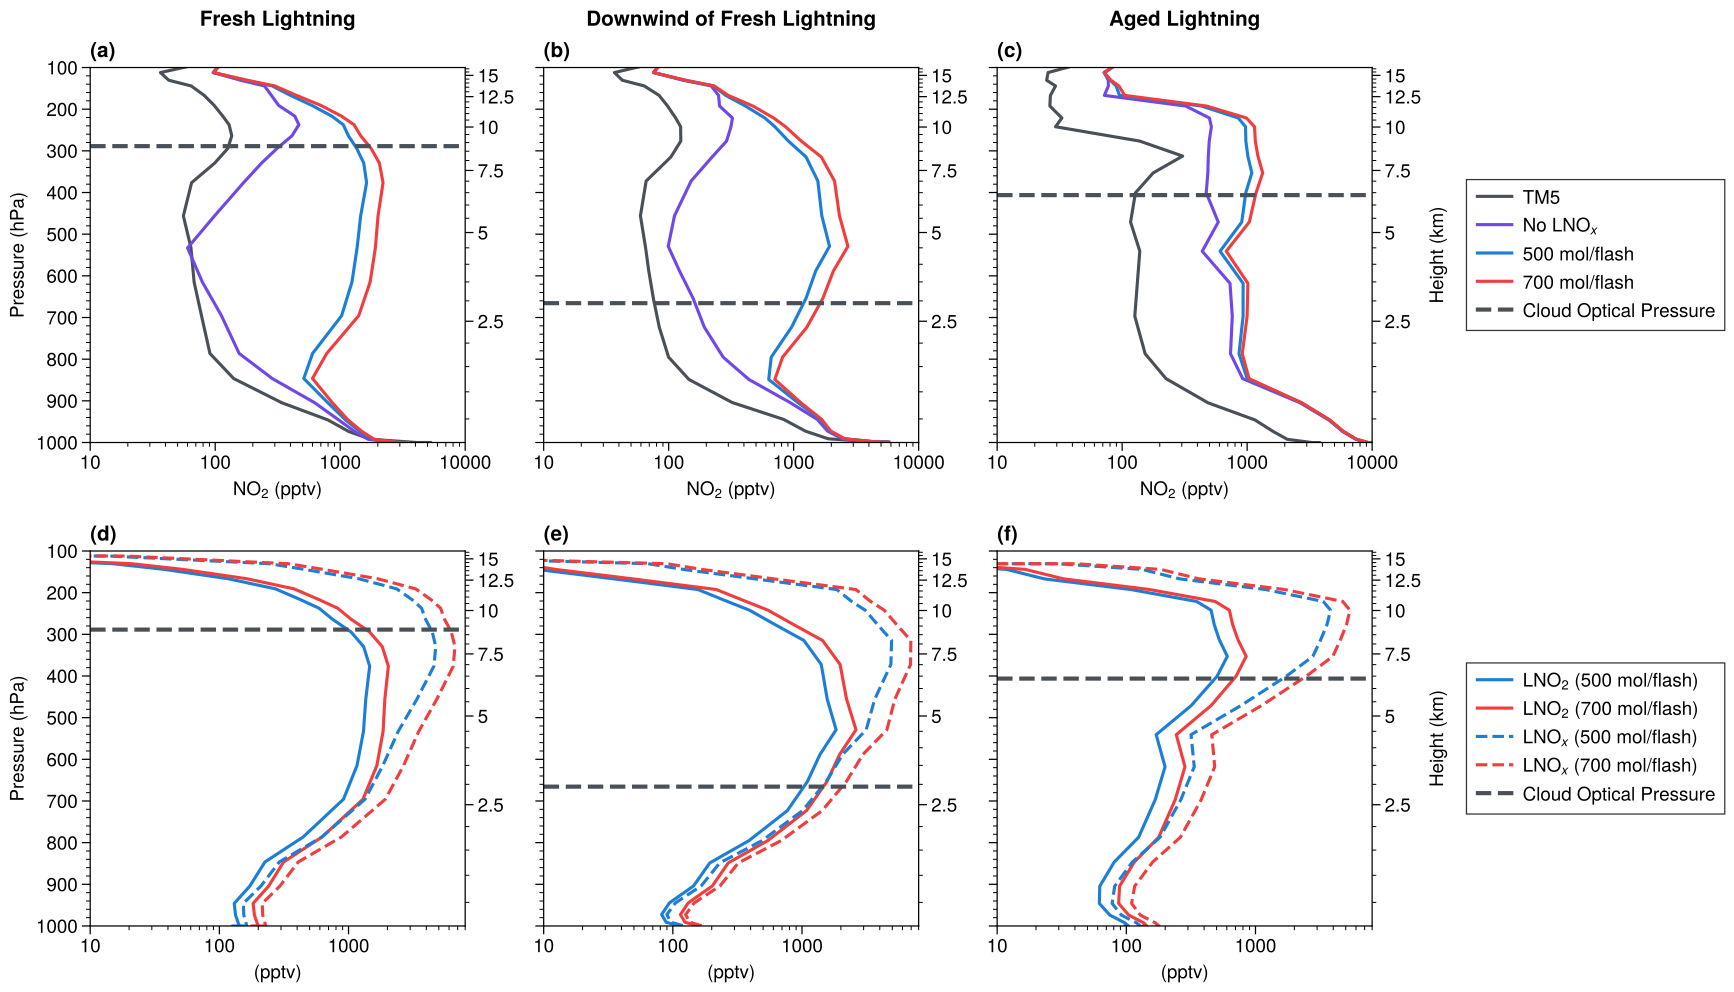
\includegraphics[width=0.8\columnwidth]{./figures/china_nox_profile.png}
    \caption{
    TROPOMI过境时在不同闪电NO的排放条件下,三个区域(新生闪电区、闪电下风向和闪电老化区)的各物质垂直廓线。
    (a--c)NO$_2$廓线与官方TM5先验NO$_2$廓线之间的比较。
    (d--f)在不同闪电NO产率设置的条件下,LNO$_2$ 和 LNO$_x$之间的廓线分布比较。灰色虚线是TROPOMI探测到的云压。\\
     Figure \ref{fig:china_nox_profile}. Profiles with different lightning NO productions at TROPOMI overpass time over three regions (fresh lightning, downwind of fresh lightning, and aged lightning).
    (a--c) The NO$_2$ profiles compared with the official TM5 a priori NO$_2$ profile.
    (d--f) The comparisons between LNO$_2$ and LNO$_x$ profiles with different lightning NO production settings.
    The gray dashed line is the cloud optical pressure detected by TROPOMI.
    }
    \label{fig:china_nox_profile}
\end{sidewaysfigure}


\begin{figure}[H]
    \centering
    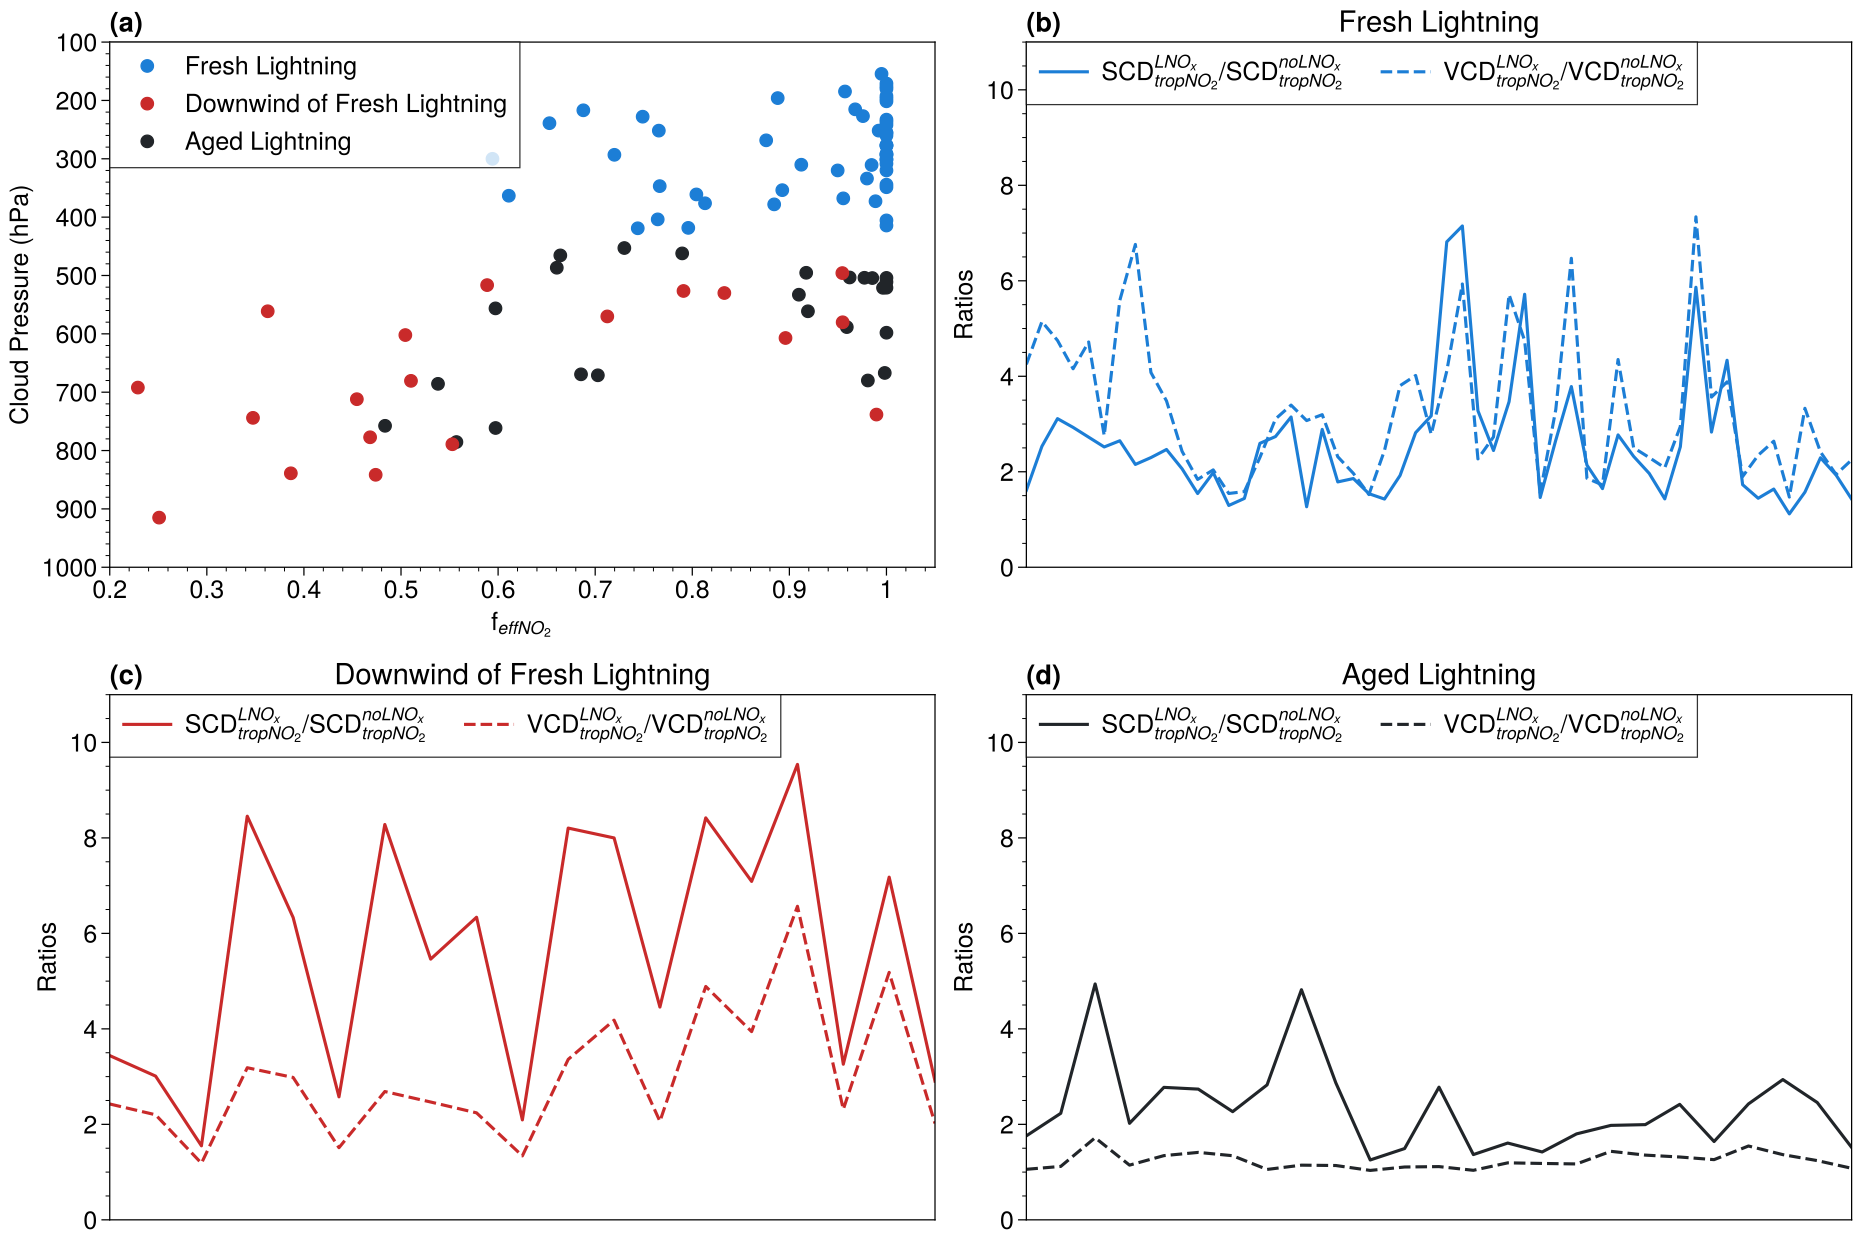
\includegraphics[width=0.9\textwidth]{./figures/china_amf_contribution.png}
    \caption{
    (a)图 \ref{fig:china_s5p_amf_diff} 中定义的三个区域(新生闪电区,闪电下风向,和闪电老化区)的云压和云辐射分数之间的关系。
     (b--d)这三个区域的先验SCD$^{\textrm{LNO$_x$}}_{\textrm{tropNO$_2$}}$/SCD$^{\textrm{noLNO$_x$}}_{ \textrm{tropNO$_2$}}$和先验VCD$^{\textrm{LNO$_x$}}_{\textrm{tropNO$_2$}}$/VCD$^{\textrm{noLNO$_x$ }}_{\textrm{tropNO$_2$}}$。
     LNO$_x$的上标表示先验变量是通过开启LNO$_x$排放(每次闪电 500 mol NO),而上标为noLNO$_x$代表关闭LNO$_x$排放。\\
     Figure \ref{fig:china_amf_contribution}. (a) The relationship between cloud pressure and cloud radiance fraction for three regions defined in Fig. \ref{fig:china_s5p_amf_diff}: fresh lightning region, downwind of fresh lightning, and aged lightning area.
    (b--d) The a priori SCD$^{\textrm{LNO$_x$}}_{\textrm{tropNO$_2$}}$/SCD$^{\textrm{noLNO$_x$}}_{\textrm{tropNO$_2$}}$ and a priori VCD$^{\textrm{LNO$_x$}}_{\textrm{tropNO$_2$}}$/VCD$^{\textrm{noLNO$_x$}}_{\textrm{tropNO$_2$}}$ of pixels in these three regions. The LNO$_x$ superscript indicates that the a priori variable is calculated with LNO$_x$ (500 mol NO per flash) and the noLNO$_x$ superscript is without LNO$_x$.
    }
    \label{fig:china_amf_contribution}
\end{figure}


\section{本章小结}

本章基于不同云高条件下卫星遥感的云上NO$_2$柱浓度,利用云切片方法得到对流层顶--330 hPa、330--450 hPa、
450--570 hPa、570--670 hPa、670--770 hPa和770--870 hPa间的NO$_2$平均浓度。
云切片得到的NO$_2$廓线可用于评估全球化学模式,并为对流输送、平流扩散和LNO$_x$排放的开发提供参考。
我们将TROPOMI的云切片结果与MERRA2-GMI和TM5模式的对流层 NO$_2$ 廓线进行了比较,主要结论如下:

\begin{enumerate}[label=(\arabic*), labelindent=\parindent, leftmargin=0pt, widest=0, itemindent=*, topsep=0pt, partopsep=0pt, parsep=0pt]

\item TROPOMI的云切片结果表明,陆地上对流层顶--330 hPa间的NO$_2$浓度为450--570 hPa间的$\sim$2倍,570 hPa以下的NO$_2$浓度逐渐上升,
即云内的NO$_2$廓线呈“C”型,说明LNO$_2$ 在对流层上层占主导,而污染 NO$_2$ 在对流层下层占主导;

\item 进一步分析了TROPOMI数据与MERRA2-GMI和TM5模式结果之间的误差分布情况,
结果表明,模式中LNO$_2$排放或参数化对流垂直传输污染物的强度可能偏低,
导致其在污染地区的对流层上层[对流层顶--330 hPa和330--450 hPa]的模拟结果比TROPOMI观测值低10--50\%。
而在对流层中层和低层,由于MERRA2-GMI使用的排放清单未及时更新,
导致污染地区(尤其是中国东部和印度北部)的NO$_2$模拟平均浓度为TROPOMI观测值的$\sim$2倍。

\item 将设置不同LNO$_2$产率的WRF-Chem高分辨率结果代入TROPOMI NO$_2$柱浓度的计算,
敏感性试验结果显示,若考虑LNO$_2$的贡献则AMF$_{\ch{trop}}$在新生闪电区会降低23\%,而在出流区和老化区会增加60\%。

\end{enumerate}
